\documentclass{xduugthesis}
\usepackage{bookmark}
\usepackage{pgfplots}

\xdusetup{
	style = { 
		cjk-font = win, 
		latin-font = tac,
		bib-backend = biblatex,
		after-skip = {18pt,12pt,12pt,12pt,10pt,10pt},
		before-skip = {20pt,14pt,14pt,14pt,12pt,12pt}
	},
	info = {
		title = {
			基于RecyclerView的高性能\\Feed流研究与应用
		},
		author = {赵传博},
		major = {软件工程},
		supervisor = {王琨},
		department = {计算机科学与技术学院},
		abstract = {chapter/abstract.tex},		% Chinese abstract
		abstract* = {chapter/abstract_en.tex},	% English abstract
		class-id = {2003052},
		student-id = {20009200303},
		bib-resource = {bibres/cites.bib},
		keywords = {安卓, 性能优化, 绘制, 应用开发},
		keywords* = {Android, Performance Optimization, UI, Application Development},
		acknowledgements = {chapter/thanks.tex}
	}
}
\begin{document}
\chapter{绪论}

\section{研究背景及意义}

Android 是目前使用非常广泛的系统\cite{businge2019studying}。无论是手机、平板、电子书、车机还是嵌入式设备等都在运行 Android 系统。Android 应用程序的开发和迭代也的速度也在日益增加。随着代码不断累积,应用本身的业务逻辑也越来越臃肿。因此需要对应用的主要业务场景不断优化,才能削减业务代码增加带来的性能方面的负面影响。

Android 系统的大部分 UI 绘制是交由应用的主线程来执行\cite{yan2014real}。主线程从 ActivityThread 的 main 方法开始运行,通过消息机制来不断处理 UI 的绘制消息和应用内部在主线程执行的业务逻辑,从而让应用运行下去,并响应用户的操作行为而进行 UI 上的改变。在这个过程中,如果主线程进行了过多的操作导致消息不能及时处理,就会发生卡顿,从而让 UI 不能及时刷新,影响用户的体验。因此需要对主线程的代码进行不断优化和解耦,让 UI 操作及时得到处理。

目前绝大部分 Android 应用的主要场景是一个信息流,来给用户呈现最新的推荐信息。这些信息包括但不限于视频、新闻、帖子等流式信息。这些信息的刷新和展现大部分也都是由主线程来完成。而作为一个应用的主要场景,甚至是应用的门面,这些场景的业务代码通常更新频率非常高,业务逻辑迭代也会非常快,导致这些场景的代码的劣化速度也远高于其它场景。所以,这部分代码对流畅性的影响是要尽可能削减的。

这些流式信息为了方便用户浏览,通常也都会用流式布局来承载。其中应用最广泛的就是 RecyclerView,一个高性能的流式布局容器\cite{sabiyath2020enhanced}。当用户在 RecyclerView 中快速滑动时,它会根据目前的情况合理分配和回收每一个子项目的引用和视图,从而减少其在内存和性能方面的整体开销。然而,随着业务代码的不断积累,RecyclerView 本身带来的性能收益也会逐渐被淹没,同时 RecyclerView 也已经承载了太多的业务逻辑,很难在短时间内深度解耦。因此本文尝试从另一个角度针对特定的业务场景进行深度优化,从而提高用户的流畅性体验。

基于 RecyclerView 的优化对于整个 Android 应用的性能大盘提升甚至是用户增长都有很重要的意义。由于用户的消费时长几乎都在应用的 Feed 流中,并且应用本身的流畅性的提高也有利于用户持续进行消费而不是中途退出,因此即使是比较小的性能提升,折算在 Feed 场景中也能得到很大的收益。在本文中,具体开展的 Feed 流优化工作是针对数据绑定阶段的。在优化后,数据绑定阶段会尽可能避开用户触发的滚动事件,通过量化的指标可以观察到该优化极大地提升流用户的流畅性体验。

\section{国内外研究现状}

目前国内外对于 Android 应用流畅性优化的工具和检测手段有很多。以谷歌官方为例,在 RecyclerView 的渲染流程中,提供了用于数据异步加载的 AsyncListUtil 工具,用于增量刷新的 DiffUtil 工具,同时也在 RecyclerView 内部集成了很多性能优化的轻量组件。针对流畅性监控以及一些常见的性能优化场景,国内的很多互联网企业也贡献了许多开源的项目。如腾讯的 Matrix,快手的 KOOM,字节跳动的 RheaTrace 等等。合理地利用这些检测和优化工具,能够快速定位需要优化的场景,并迅速将一些常见的优化手段落地,从而评估整体的优化空间和收益。

目前针对应用 Feed 场景的公开优化手段非常有限,尤其是业务高度复杂的 Feed 流场景。而这部分场景恰恰也是用户感知最强烈,最能影响用户整体流畅性体验的场景。通过在实习单位中进行内部调研,发现这部分的优化对于一些用户量庞大、业务结构复杂的互联网应用来说是非常关键的,同时也已经有非常多的优化策略在内部流行。然而,以流畅性优化为例,这些对内的优化场景大多与应用本身的业务逻辑高度耦合,很难做到框架级别的封装。即使能够做到,对于 Android 设备的支持广度也相当有限。

\section{本文的主要工作介绍}

本文致力于针对 RecyclerView 数据绑定这个细化但核心的场景进行优化。设计一个轻量化的预渲染框架,能够让 RecyclerView 的数据绑定避开其它的耗时逻辑,从而优化用户在滑动过程中的整体流畅性。

为了能够量化优化的结果,还需要一些手段来验证。其中最复杂的部分就是如何找到采集指标信息的时机,并在这个时机进行信息的收集。最普遍的手段就是采集帧率指标,然而目前业界内的帧率采集手段依然有一些不足。所以也要探究出一个更加准确的帧率采集手段,并在这个基础上,继续探索其它的性能指标来衡量对于 RecyclerView 的其它方面做出的优化成果。

最后,不只局限于视频类型的应用,RecyclerView 更多被应用于以大量图文为基础的信息流。针对这种场景也需要进行一定程度的优化,并通过其它方面的量化指标来衡量优化的效果;同时也设计了一个秒开检测框架来收集相应的性能指标。

\section{本文的结构安排}

\begin{itemize}

    \item 相关技术与理论基础:由于业界并没有详细的针对 RecyclerView 的解析,同时本文的优化需要在其基础上对核心部分进行修改,所以为了避免对业务方产生影响,需要对 RecyclerView 以及 Android 整体的绘制体系进行深度调研。在有了这些知识储备的情况下,才能尽可能全面地排查出优化中产生的副作用。本部分对应第 2 章。

    \item Feed 流优化工作:接下来,会介绍预渲染框架具体应用场景的背景、预渲染技术方案的选型、框架的总体设计思路和细节实现、开发过程中遇到的问题和解决过程。同时该项目也已经在实习公司内经过一轮完整的需求提出、需求评估、需求开发、缺陷修复、灰度测试、线上通过实验验收的流程。同时,针对一些以图文为主的 Feed 流场景的流畅性优化,也进行了简单的调研和开发。本部分对应第 3 章。

    \item Feed 流优化验证:最后,是对于这些优化手段的验证。通过设计的框架收集性能指标,从而验证优化的结果。同时,为了能够模拟真实的 Feed 流场景,还开发了一个简单的 Feed 流用作优化目标。本部分对应第 4 章。

\end{itemize}

\chapter{调研工作与源码解析}

对于 Android 应用中图形的绘制体系的优化,需要深度对底层源码进行调研,然后才能上手进行优化。因此开展了流畅性优化调研工作,阅读 Android Framework 以及 Android SDK 的源码,总结出整体的应用绘制体系。在有了这些前置知识的情况下,进行针对 RecyclerView 的优化工作,并搭建合理的流畅性指标来量化优化结果。具体来说,需要对 Android 的绘制体系 —— View 有一定的了解;同时对于 Android 应用对触摸消息的处理以及 Android 消息机制也要有所了解。这些都是 Android 应用程序运行的根本。

\section{Android 绘制体系}

\subsection{View 的测量、布局和绘制}

在 Android 应用程序中,展示 UI 界面以及和用户进行交互的最主要的组件就是 View。View 本身是一个非常复杂的绘制框架,封装了一系列与屏幕刷新相关的操作。开发开发者可以使用 Android SDK 中提供的 View,或者针对具体的业务自定义一些 View 来进行界面的展示,业务逻辑交互的处理操作。对于一个 View 来说,最重要的生命周期有测量(measure)、布局(layout)和绘制(draw)\cite{rountev2014static}。

在测量的过程中,需要确定每一个 View 所占据的矩形区域的大小。其中最典型也是最耗时的就是文本类型的 View 的测量。这些文本因为语言、字符宽度、文字方向等不同的因素,需要进行非常复杂的测量流程,最终才能确定文本的长和宽。因此,View 的测量流程通常也是 View 进行绘制的时候最耗时的一个过程。

在布局过程中,需要根据每一个 ViewGroup 规定的布局方式对其中的子 View 进行布局,也就是确定其在 Window 上显示的位置。常见的 ViewGroup 有线性布局 LinearLayout,帧布局 FrameLayout和相对布局 RelativeLayout 等。这些不同的布局对于其中的子 View 有不同的布局要求,并在真正布局的时候按照这个要求确定子 View 应该摆放的位置。

最后一步就是绘制了,也就是真正将图形绘制到屏幕上的操作。这部分工作大部分是通过 Android 的上层渲染组件 Canvas 来完成的。 Canvas 会将各种类型的图形在 CPU 上进行计算,之后会将这些计算好的结果发送给 GPU 进行渲染。这也是大部分 Android 动画实现的原理。

\begin{figure}
    \centering
    \begin{adjustbox}{max width=\textwidth}
        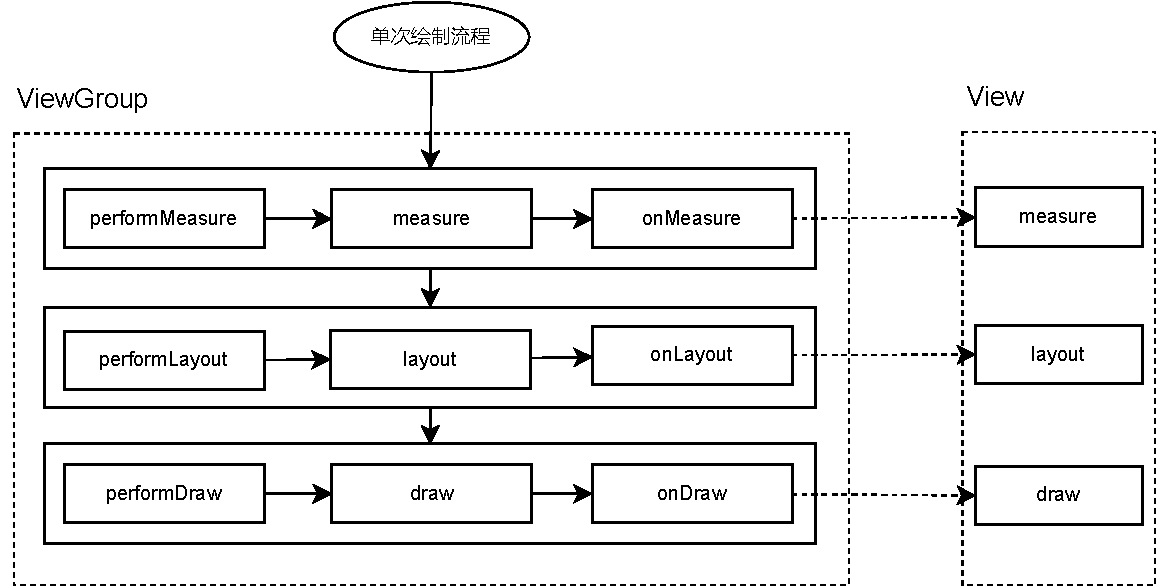
\includegraphics{assets/view-measure-layout-draw.pdf}
    \end{adjustbox}
    \caption{View 的绘制流程}
\end{figure}

对于 ViewGroup 来说,测量的流程需要特别强调。因为 ViewGroup 本身没有内容,它的作用是承载子 View。所以,ViewGroup 的主要测量过程就是去测量自己的子 View,并最终得到所有子 View 的综合属性。大致的 ViewGroup 与 View 配合进行绘制的流程见图 2.1。

然而,View 体系并没有限制 ViewGroup 应该在测量的时机一定得到子 View 的准确测量结果。这就意味着我们可以在测量的时候返回一个假值,并在后面的时机得到真正的值。RecyclerView 就是这样做的。因为它通常需要承载大量的子 View,因此它对于性能的要求非常高。所以它的测量流程作为非常耗时的一个流程,需要尽可能地减少测量的总次数以及避免重复测量。RecyclerView 真正测量子 View 是在布局流程中,在测量完子 View 之后会立刻对子 View 进行布局。这种方式能够避免子 View 在不适宜的时机请求父 View 测量而导致性能下降的问题。当 RecyclerView 在进行布局时,它会禁止子 View 进行布局请求,从而拦截子 View 的测量请求,从而减少不必要的测量次数。

% 这部分之后会在 4.2 详细说明。

\subsection{用户输入事件的处理}

当用户用手触摸屏幕时,触摸行为会定位到特定的 View 上。但是,这个触摸行为只会在下一帧到来时进行响应。因为受限于屏幕的刷新率,只有在下一帧屏幕才能给出新的图像。触摸事件主要有以下几种:

% 所以等到 Choreographer 接收到下一个 VSync 信号时,新的绘制流程启动,这些积累的触摸事件就会在这个时候被消费。

\begin{itemize}
    \item ACTION\_DOWN:用户手指按在屏幕上的事件;
    \item ACTION\_MOVE:用户手指在屏幕上滑动的事件;
    \item ACTION\_UP:用户手指从屏幕上抬起的事件;
    \item ACTION\_CANCEL:当事件被上层 ViewGroup 拦截之后,下层 View 接收到的事件。
\end{itemize}

\begin{figure}[htbp]
    \centering
    \begin{adjustbox}{max width=\textwidth}
        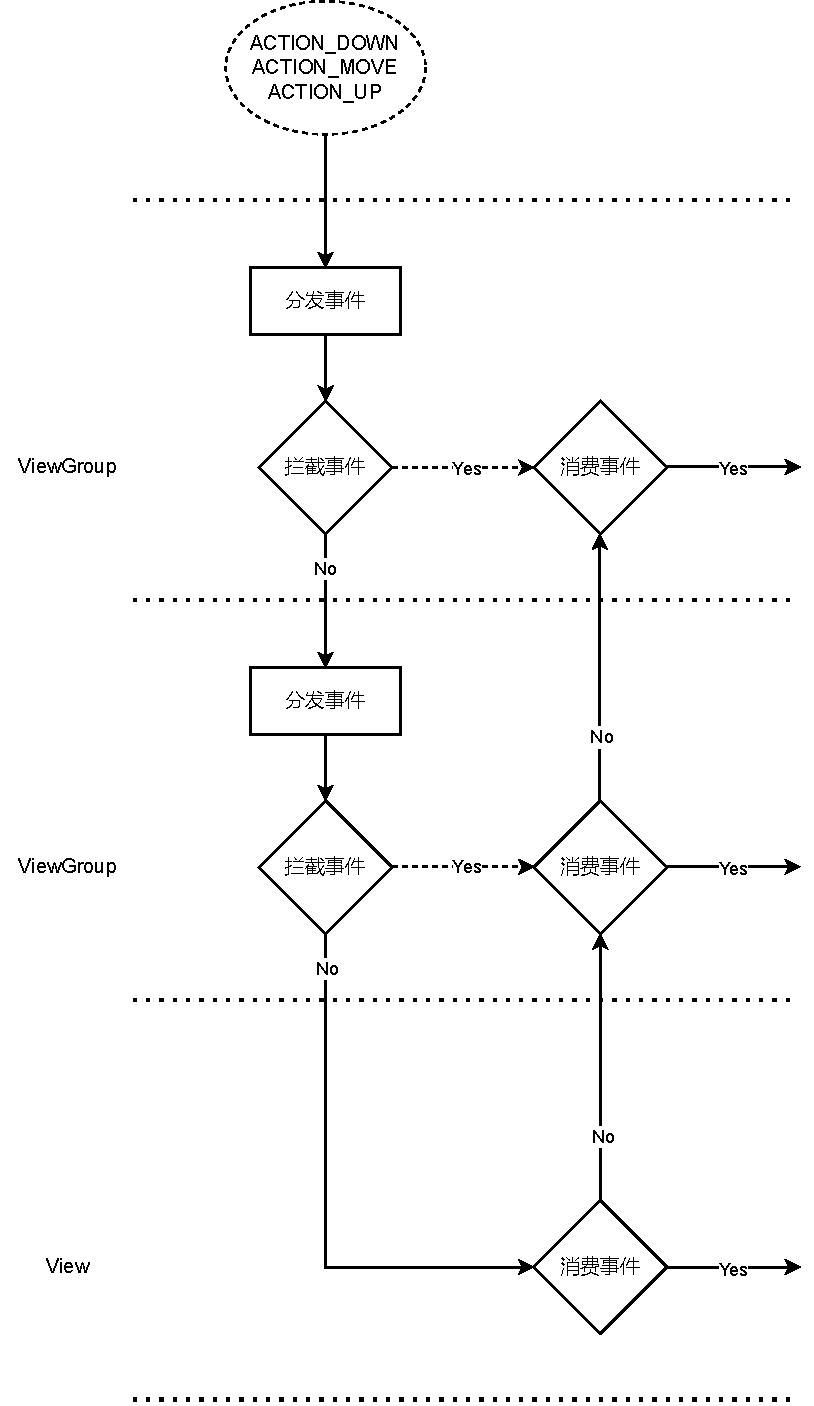
\includegraphics[scale=0.7]{assets/view-touch-event.pdf}
    \end{adjustbox}
    \caption{View 的触摸事件传递流程}
\end{figure}

触摸事件会从 View 树的根节点开始向下传递。事件在链路中流动的路线总体上呈现出“U 型”,如图 2.2。在从顶层的 View 开始向下进行事件的分发(Dispatch)。在这个过程中,路径上的每一个 ViewGroup 都可能拦截(Intercept)这个事件\cite{wu2017appcheck}。如果事件已经传递到了最底层的 View,又或者被其中的某一个 ViewGroup 成功拦截,那么将会由相应的 View 或者 ViewGroup 去逐一消费这个事件。如果事件被当前 View 或 ViewGroup 消费,那么事件的传递将在此终止;如果没有被消费,那么事件会向上传递,直到再次传递到根 View 为止。

对于 RecyclerView 来讲,因为其需要处理大量的滚动操作,所以触摸事件的处理尤为重要。当触摸事件被 RecyclerView 拦截时,它会通过当前是否是滚动状态而选择是否拦截该事件。如果是 ACTION\_MOVE 事件,RecyclerView 通过解析事件的详细信息,发现此时用户触发了滚动操作,那么就会将自己标记为滚动状态,并最终拦截这个 ACTION\_MOVE 事件。因此,之后的事件消费也是由 RecyclerView 自身来进行(嵌套滚动不适用于这段说明,但其不在本文的讨论范围内);如果是 ACTION\_DOWN 事件,那么 RecyclerView 不会拦截这个事件,让其成功到达子 View,由子 View 来决定是否消费该事件。这个过程中,子 View 是否消费 ACTION\_DOWN 事件对后续的事件传递影响尤为重要。如果处理不当,可能会产生一些影响很重大的缺陷。

% 这部分会在 5.4.1 详细说明。

\subsection{Android 消息机制}

Android 应用程序运行的基本框架就是基于消息机制,同时绘制行为和消息机制的配合也非常紧密。Android 系统应用内部的消息机制主要和这几个类相关:Looper、Handler 和 MessageQueue。

Android 系统的主线程对应的类是 ActivityThread。该类内部维护着主线程启动,并处理各个线程发送消息的流程,同时也负责 UI 的绘制消息的处理。当该线程启动时,同时会准备自己的 Looper 来负责消息队列的管理和任务的委派。ActivityThread 中的 Looper 成为 Main Looper。由于只能由主线程来处理 UI 类型任务的分发,所以 Main Looper 也只允许主线程持有。如果应用内部的线程也想利用这套消息机制来进行任务处理(比如埋点上报的线程),也可以准备自己的 Looper 来接收任何线程发送给当前线程的任务并添加到消息队列中,在某一个时刻被取出并执行。

Looper 内部管理的消息队列的实现类就是 MessageQueue。其内部管理了任务队列的管理操作,包括入队、出队,以及空闲时的敏捷任务处理操作等。大部分是通过调用 Android Native 的 C++ 代码来实现,并通过 JNI 包装成面向 Android Framework 以及 Android 应用程序的接口。

Android 程序中,消息不能直接通过访问 Looper 或者 MessageQueue 的方式进行提交,只能通过封装好的方式 —— Handler 进行提交。这种方式更加安全和方便,也能给应用的架构设计提供更好的开发范式。在任何线程中都可以创建 Handler,但是 Handler 在构造的时候必须指定 Looper,也就是明确提交的任务需要由哪一个线程的 Looper 来管理\cite{fan2018efficiently}。同时,Handler 也提供了多种任务执行的方式、多种提交任务的方式以及延时和取消等功能。例如,我们可以在发送一个任务之前,取消之前已经提交但未执行的特定类型的任务来满足特定的业务需求。在对 RecyclerView 的布局流程进行改造时,我们也会利用到这一特性。

\section{Feed 流概念及现状}

目前,越来越多的互联网产品在移动端上增加“短视频”功能,如快手、抖音、美团、西瓜视频、小红书等等,并且短视频板块在这些应用中通常都处于启动的默认引导场景,即 Feed 流,是整个应用平均消费时间最长的板块。因此,这部分的流畅性体验对于用户的留存,消费时长等指标至关重要。能够优化视频起播的速度、滑动的流畅度、网络请求速度等任何一个场景,都能带来非常大的业务收益。本节主要针对基于 RecyclerView 搭建的短视频场景的 Feed 流进行流畅性的优化。因此,首先需要对 RecyclerView 的具体情况进行调研,才能从中找出可以优化的点。

\subsection{RecyclerView 介绍}

RecyclerView 最早在 Google I/O 2016 被提出,用来解决传统应用程序中使用 ListView 处理复杂的列表时带来的性能问题。RecyclerView 本身也是一个 ViewGroup,与其它常用的 ViewGroup,如 ScrollView、ViewPager、ListView 等在绘制流程中的行为是几乎一致的\cite{mawlood2022listview}。只不过,RecyclerView 更加专注于在流式布局的场景下,对于多种复杂的子项进行合理的回收和复用,从而在不断滑动的过程中,增加已有组件的利用率,提高滑动时的性能和流畅度。

RecyclerView 不是单独的一个组件。由于处理各种子 View 的回收和复用,以及处理动画、数据绑定等操作的逻辑都非常复杂,因此将这些逻辑都分成独立的部分。整个 RecyclerView 家族主要由以下几个组件组成:

\begin{itemize}
    \item RecyclerView:父 View 本身,负责响应原有的 View 绘制流程,作为其它组件行为的发起者;
    \item LayoutManager:负责 RecyclerView 的测量和布局流程,安排子 View 的位置。有不同的实现方式,比如线性布局,网格布局等等。本文中主要考虑在 Feed 流场景下常见的线性布局 LinearLayoutManger;
    \item ItemAnimator:负责子 View 的显示,隐藏等动画。因为不涉及到核心的布局流程,所以本文不涉及到这方面的优化;
    \item Adapter:RecyclerView 最核心的数据管理类。所有的子 View 中的数据由 Adapter 来管理,并在合适的时机进行绑定,从而能够显示在屏幕上。Adapter 作为数据的存储器,能够通知 RecyclerView 数据发生了何种变化,从而通知 RecyclerView 进行适当的刷新操作。
\end{itemize}

接下来将通过对 RecyclerView 本身的测量、布局、滑动、数据处理流程来认识这些组件,并引出相应的优化点。

\subsection{RecyclerView 的测量}

对于一个 ViewGroup 来说,它的测量过程就是要知道自己所有的子 View 的综合属性。然而,如果 RecyclerView 本身无法知晓子 View 都有谁,那自然无法进行测量。和其它的布局(如 LinearLayout,FrameLayout 等)不同,其它的布局在创建的时候,无论是通过 XML 还是手动在代码中调用 addView() 来创建,都是已经知道子 View 的完整状态;而 RecyclerView 获取子 View 参数信息的手段是通过 Adapter。而 Adapter 最重要的数据准备过程是交给开发者来决定的。因此,在初次测量时,RecyclerView 拿不到任何子 View 的信息。这个时候,如果RecyclerView 在布局方向(垂直或水平)上的属性是固定的值,那么测量就会很简单,直接返回对应的值即可;如果是一个不确定的值(比如 WRAP\_CONTENT),那么会先尝试进行一次布局流程,然后再进行测量。通常情况下, RecyclerView 在布局方向上的长度都是一个固定的值,因为这样能够很大程度上减少重复测量的次数,从而提高滑动的性能。

\subsection{RecyclerView 的布局}

布局是 RecyclerView 最关键的流程。这里涉及的就是对Adapter的消费,布局其中的子 View,以及回收和复用发生的地方。布局操作的整个流程在方法 dispatchLayout() 中,里面的流程分为三步。这三步所做的事情如下:

\begin{itemize}
    \item 第一步:处理 Adapter 中提交的更新,同时保存当前子 View 的参数信息;
    \item 第二步:对于每一个子 View,执行最终的测量和布局流程,确定它们安放的位置。这个过程也是 RecyclerView 和 Adapter 交互最主要的过程 —— 进行数据绑定;
    \item 第三步:主要处理动画的流程。因为不涉及到布局上的性能优化,本文不进行讨论。
\end{itemize}

接下来,我们将对 RecyclerView 最主要的布局流程进行分析。首先,RecyclerView 会拦截子 View 对布局的请求。在 RecyclerView 布局的过程中,子 View 本身就已经将要被布局,因此 RecyclerView 认为在这个时刻任何子 View 的布局请求都是多余的。RecyclerView 并不会允许子 View 在这个时候请求布局。等到第三步结束之后,才再次允许子 View 进行布局请求。实际上,在真实开发过程中,也非常不建议在 RecyclerView 的子 View 中手动进行布局请求,而是使用 Adapter 去通知的方式进行增量更新。这样会有更高的效率和更安全的执行流程。

核心布局流程可以简单概括为:计算出起始锚点(通常是延布局方向的起始位置),并沿着布局方向决定每个 View 的行为。有可能是创建新的 View,也有可能是复用之前回收的 View;并给这些确定会显示在屏幕上的 View 进行数据绑定。这个过程中,创建和绑定的操作是交给 Adapter 来完成的。也就是说,开发者需要在自己的 Adapter 中完成创建和绑定的流程。因此,这个过程中我们能够进行一些特殊的操作。比如提前拿到 View 进行绑定,甚至利用空闲时间异步创建出 View 来避免真正用到 View 时才去创建而导致耗时增加;另外要强调的一点是,由于 View 本身不能具有 RecyclerView 需要的准确的参数信息(位置信息,状态变化标记位等),同时也不能被妥善地回收和复用。因此 RecyclerView 框架的做法是在 View 上包装一层 ViewHolder 来持有 View 的引用。对于 LayoutManager 来说,它直接操作的是 ViewHolder 而非 View,这样能够更好地对 View 进行回收和复用,也便于增加一些位置变化等关键信息来让 LayoutManager 更迅速地进行布局操作。

% \subsection{RecyclerView 对于滑动过程的处理}

% 任何 View 处理滑动流程时,都需要处理 ACTION\_DOWN 事件、ACTION\_MOVE 事件和 ACTION\_UP 事件。通常,一个完整的滑动流程是一个 ACTION\_DOWN 加上若干个 ACTION\_MOVE 以及结尾的 ACTION\_UP。因此,对于 RecyclerView 来说,如何处理 ACTION\_DOWN 事件的走向尤为重要,这影响了后续事件的分发,自然也影响了整个的滑动流程。当 ACTION\_DOWN 事件产生时,RecyclerView 并不会拦截该事件,只会将事件传递给子 View。而子 View 可以自主选择是否消费该事件。如果子 View 没有消费 ACTION\_DOWN,那么将会由 RecyclerView 自己来消费。RecyclerView 本身永远会消费任何触摸事件,所以无法再继续向上传递。之后所有的 ACTION\_MOVE 事件以及最后的 ACTION\_UP 事件都会由 RecyclerView 自己来消费。这也是滑动流程中最理想的情况,完全由 RecyclerView 来主动控制。

% 但是,通常 RecyclerView 的子 View 是需要消费 ACTION\_DOWN 事件的。比如一个可以点击的新闻条目、一个视频条目等等。这些响应了点击事件的子 View 自然需要消费 ACTION\_DOWN 事件来处理点击过程。这也就导致了接下来的 ACTION\_MOVE 事件并不会被发送给 RecyclerView 来消费。那么在这种情况下,RecyclerView 应该如何处理滑动流程呢?答案是通过拦截。虽然 RecyclerView 接下来不会收到子 View 传递来的未经过消费的 ACTION\_MOVE 事件,但是在将其传递给子 View 之前,RecyclerView 本身也可以拦截该事件。因此,RecyclerView 在拦截的流程中,只要发现当前事件是 ACTION\_MOVE 事件,就会设置滑动状态的标记位,并拦截该事件。结果就是子 View 会收到 ACTION\_CANCEL 事件从而无法进行滑动处理(不进行嵌套滑动处理的条件下),而 RecyclerView 本身能够通过该方式消费 ACTION\_MOVE 事件以及最后的 ACTION\_UP 事件。虽然这样确实能够保证 RecyclerView 正常处理滑动流程,但是和直接处理不同,如果是通过拦截的方式处理 ACTION\_MOVE 事件,拦截的过程和真正进行滑动的过程会位于两个不同的消息,也就是两个不同的流程中。这样会导致如果中间被其他消息插入,会产生一些副作用。这部分也是我们在优化过程中需要重点克服的困难之一。

% 在真正进行滑动的过程中,会对每一次滑动事件进行解析。解析出的滑动距离、方向等属性会用于接下来的布局过程。RecyclerView 会对因为滑动而改变的子 View 进行重新的测量和布局,并尽可能复用已经被回收的 ViewHolder 来减少重复创建。对于新添加的子 View,也会通过 Adapter 进行数据绑定。

\subsection{RecyclerView 对数据改动的响应}

RecyclerView 最推荐的方式是进行增量更新,而不是全量更新。全量更新会导致 RecyclerView 整体的刷新,同时会将所有已经位于屏幕上绑定数据完成的 View 进行回收和废弃,接下来会重新用新的数据进行绑定。因此,如果真正的修改只有非常小的一部分,建议通过增量更新的方式通知 RecyclerView,之后在 RecyclerView 的布局阶段的第一步中会消费这些更新请求,并在最终布局的流程中只进行修改部分的重新布局。这对于性能的提升很大,同时也为动画的执行留足了 CPU 资源。

数据改动的通知是通过 Adapter。当需要的数据发生变化时,会先修改 Adapter 持有的数据结构,并调用 Adapter 的接口去通知 RecyclerView 发生了什么样的变化。这些改动统一被包装成接口,调用即可提交改动至 RecyclerView。而 RecyclerView 本身通过观察者模式观察 Adapter 中的数据变化。每一次改动行为都会被存放到队列中进入代办(Pending)状态,直到布局流程开始时会被消费。在消费的过程中,也只会通过改动中提交的位置信息对可能受影响的子 View 进行修改。

\subsection{视频类型 Feed 流}

在视频类型 Feed 流的场景下,通常 RecyclerView 的一个子 View 作为一个视频的载体。当用户向下滑动时,下一个视频由于被滑动到屏幕内,会进行布局和数据绑定,从而显示在屏幕上。这里面主要的信息有视频的封面图片、视频标题、作者信息等等。从用户的感官角度看,当该子 View 被滑动到屏幕中央定位完毕时,视频会进行播放,此时用户可以对视频的进度,播放速度等进行控制。同时能够通过点赞、评论、收藏等方式进行交互。

% 对于下一个视频信息的加载过程,通常是需要格外小心的。因为该过程发生在用户滑动屏幕的时候,此时主线程正不断接受用户发送的滑动事件,并根据这些滑动的事件来进行布局、UI 刷新等操作,占据了主线程很大一部分资源。如果这个时候数据绑定的流程过于复杂,会严重增加这段时间的主线程耗时,从而影响整体的流畅性,甚至造成肉眼可见的卡顿。因此,在 Adapter 进行数据绑定的过程中,是强烈不建议在主线程进行任何耗时任务的。这些任务要么通过异步的方式后续补齐,要么针对具体的业务,寻找合适的时机提前进行。

% 然而,经过业务的不断迭代,数据绑定的耗时一定会随着业务方不断添加新的功能而增加。因此,我们希望能够对这个过程进行彻底的优化。也就是能够在一个合适的时机将整个数据绑定操作提前进行,而不是只异步化其中的一小部分。在视频 Feed 流的场景中,合适的时机是比较容易寻找的,因为用户在滑动到一个视频之后通常会停留一段时间进行交互行为。但是这样的行为会让 RecyclerView 的生命周期产生混乱,因此即使能够做到,也需要经过细致的修复来让其能够准确地派发原先的生命周期。

通过对公司内的线上应用,传统的利用 RecyclerView + SnapHelper 来开发视频类型应用的范式,以及网络上开源的视频应用开发手段得出,基于 RecyclerView 所搭建的视频类型 Feed 流,通常需要进行如下定制:

\begin{enumerate}
    \item 将 RecyclerView 的缓存关闭,因为会影响生命周期派发,导致业务埋点上报混乱;
    \item 将 LayoutManager 的预取功能关闭,该功能会影响数据绑定的生命周期派发。
\end{enumerate}

接下来详细说明这两个功能需要关闭的原因。RecyclerView 的缓存机制是一种对离开屏幕的数据的暂时保护。当一个子 View 因为滑动而脱离屏幕可见范围时,理论上应该被回收,并用于接下来新出现的 View 的数据绑定。但是用户也有可能会重新向反方向滑动,让这些 View 重新显示在屏幕上。因此将这些暂时脱离屏幕的 View 放入缓存中,能够让这些数据保存下来避免被回收,这样重新显示时就不需要再次进行绑定,从而提高流畅性;然而,对于视频类型的应用来说,用户向上滑动的操作数量会少很多,反映到数据上就是 RecyclerView 的缓存命中率非常低。同时,由于增加了缓存,在 View 重新显示时不需要进行数据绑定,开发者也没有任何手段通过 SDK 获知 View 从缓存中被取出的时机。因此这些 View 的曝光埋点也就无法进行上报。所以对于视频类型的 Feed 流,缓存通常会被关闭,当 View 重新显示时依然进行绑定操作。业务方会依赖这些绑定事件,在进行数据绑定的同时上报曝光埋点,表示该子 View 已经对用户可见,代表着一次用户的消费行为;LayoutManager 的预取功能需要关闭也是同样的原因。预取会导致接下来即将出现的 View 被提前绑定,从而让曝光埋点错误上报。因为我们没有一个比较好的时机去确定当前 View 是否对用户可见,所以只能选择最接近的绑定时机。

在这样的条件下,只有当卡片因为用户滑动屏幕而出现在屏幕内时,才会进行数据绑定。这虽然能满足企业通过收集埋点来统计用户消费情况的需求,但是也会导致从用户的滑动行为开始到视图真正对用户可见的过程中出现可感知的耗时。这段时间越长,用户就越容易产生卡顿的感觉。
\chapter{预渲染框架的背景}

在视频 Feed 流中,对于下一个视频信息的加载过程通常是需要格外小心的。因为该过程发生在用户滑动屏幕的时候,此时主线程正不断接收用户发送的滑动事件,并根据这些滑动的事件来进行布局、UI 刷新等操作,占据了主线程很大一部分资源。如果这个时候数据绑定的流程过于复杂,会严重增加这段时间的主线程耗时,从而影响整体的流畅性,甚至造成肉眼可见的卡顿。因此,在 Adapter 进行数据绑定的过程中,是强烈不建议在主线程进行任何耗时任务的。这些任务要么通过异步的方式后续补齐,要么针对具体的业务,寻找合适的时机提前进行。

然而,经过业务的不断迭代,数据绑定的耗时一定会随着业务方不断添加新的功能而增加。因此,我们希望能够对这个过程进行彻底的优化。在视频 Feed 流滑动的过程中,通常用户最希望看到的是下一个视频的封面立刻展示在屏幕上。为了达到这样的目标,通用的方案有针对图片、视频参数等数据做异步加载,同时在播放器的方面也进行一定程度的预渲染。但是由于 RecyclerView 整体的刷新流程是固定的,所以数据绑定是一个必要的过程。不过在对 RecyclerView 进行了足够多的调研之后,我们可以着手进行更加深度的优化,也就是能够在一个合适的时机将整个数据绑定操作提前进行,而不是只异步化其中的一小部分。在视频 Feed 流的场景中,合适的时机是比较容易寻找的,因为用户在滑动到一个视频之后通常会停留一段时间进行交互行为。但是这样的行为会让 RecyclerView 的生命周期产生混乱,因此即使能够做到,也需要经过细致的修复来让其能够准确地派发原先的生命周期。
\chapter{问题分析和技术选型}

想要优化从滑动屏幕到用户感知卡片刷新的时间,我们不能仅仅通过正面优化绑定的行为来缩短耗时。事实上,业界内已经有一些在合适的时机进行预渲染的手段,同时也不会影响原来的生命周期分发。然而基于 RecyclerView 的 Feed 流并没有提供这样的能力。根本原因是 RecyclerView 更多还是用于处理非粘性滑动的大量图文类型的 Feed 流。因此,我们希望能够给已经在业务方面严重耦合了 RecyclerView 的 Feed 流提供预渲染的能力,提高流畅性体验。

经过调研,目前在 Android 移动端能够实现预渲染的手段主要有以下几种:

\begin{enumerate}
    \item 使用 ViewPager2 来实现预渲染,并且能够简单的封装得到完整的生命周期分发;
    \item 将 RecyclerView 的高度修改为原屏幕高度的2倍,让不可见的那部分承载预加载的 View;
    \item 通过 LayoutManager 设置额外的布局空间,从而在布局过程中多布局一部分。
\end{enumerate}

下面针对当前 Feed 流的业务场景,分析这些优化手段。首先,如果通过重构为 ViewPager2 来实现预渲染,会损失很多 RecyclerView 的灵活性,同时由于在优化项目启动时往往业务逻辑已经非常繁重,所以不可能在短时间内进行大规模的重构;而如果选择将屏幕高度修改为原来的2倍,缺点也非常明显。原本 RecyclerView 在滑动的过程中只需要维护当前 View 和新滑入的 View,在静止时只需要维护正在播放的 View。然而在修改之后需要维护的 View 个数明显增加,导致业务逻辑更加繁重,并且其它业务方(如播放器,交互,弹幕,推荐系统等)都需要做不同程度的适配。这样做的工作量也是非常大的。

因此,最终我们选择第3种方案,也就是通过 LayoutManager 提供的额外布局能力来实现预渲染。这样对 RecyclerView 本身的改动非常小,同时也只是将数据绑定的时机提前。不过,这样的改动依然会对业务造成不小的影响,所以需要对改动带来的副作用进行全方位的排查并进行适配。
\chapter{预渲染框架设计思路}

预渲染框架整体分为两部分:经过修改的 PreloadLinearLayoutManager 和派发卡片可见性事件的 ViewHolderVisibilityDispatcher。前者主要是替代原有的 LinearLayoutManager,用于实现多种模式的预渲染。同时也对一些由于预加载导致的异常情况进行了修正;后者是由于原来的数据绑定无法再被用于确定卡片是否对用户可见,从而引入的新的生命周期分发器。业务方可以通过注册卡片的可见性来进行监听,并将原来依赖于数据绑定的行为(如曝光埋点)迁移至新的回调方法中。下面对于两个组件的具体结构进行说明。

\section{实现预渲染逻辑}

LinearLayoutManager 允许提供额外的布局空间,来处理布局过程中对对超出屏幕的部分进行布局的特殊要求。方式是通过重写 getExtraLayoutSpace() 方法或者 calculateExtraLayoutSpace() 方法。其中前者只能向一个方向进行布局,后者可以在两个方向进行布局。但是,如果采用后者的话,没有引入 AndroidX 1.1.0 的项目无法使用。所以使用兼容性更强的 getExtraLayoutSpace()。

在该方法中,可以返回一个整型变量来标识需要额外布局多长的布局空间。因为我们需要额外布局一张卡片(也就是下一个视频的信息),所以返回的距离应该为一张卡片的高度。通常情况下,卡片的宽高信息可以直接通过 LayoutManager 获取到,高度通常为屏幕的高度。

通过这个简单的操作,就已经能够实现预渲染的核心逻辑,并且经过验证已经可以提前绑定下一张卡片的数据。然而,通过验证目前的生命周期,我们可以发现,这样的行为其实和没有预渲染并没有什么不同。我们通过一个例子来进行说明:当前卡片为卡片1,在这个情况下,卡片2会因为额外布局空间也被绑定并创建 View 的实例。这样确实能够达到预渲染的效果;然而,如果用户开始向下滑动,在滑动的一瞬间就会因为额外布局空间,将卡片3也提前创建并绑定。在这种情况下,依然会在滚动的过程中进行数据绑定,只不过从原来的提前一张卡片变成了提前两张卡片,耗时逻辑依然会影响主线程的性能。所以,我们需要对额外布局空间进行限制,只有在应用程序相对空闲的时刻才允许额外的布局空间。反映到业务方就是,选择一个更好的时机去进行预渲染。

为此,设计了若干种预渲染模式,来应对不同业务的需求。主要分为:

\begin{itemize}
    \item 没有预渲染(默认情况);
    \item 永远预渲染;
    \item 滚动停止时触发预渲染;
    \item 通过外界触发预渲染。
\end{itemize}

其中,通过外界触发预渲染的模式还可以分为有超时补发机制和没有超时补发机制。在有超时补发机制的版本中,当滚动停止时,如果外界没有立刻进行预渲染调用,那么就会提交一个默认为5秒的任务。当到达规定时间时外界依然没有触发预渲染,那么就会补发一次预渲染来应对一些异常情况。想要让 LayoutManager 在这些不同的预渲染模式中自如切换是需要经过缜密的设计和严谨的测试的,接下来介绍为了迎合不同的模式进行的工作。

RecyclerView 会分发滚动状态的变化。RecyclerView 的滚动状态一共有三种:

\begin{itemize}
    \item SCROLL\_STATE\_IDLE:静止状态;
    \item SCROLL\_STATE\_DRAGGING:滚动状态,不过是用户将手放在屏幕上时;
    \item SCROLL\_STATE\_SETTLING:滚动状态,用户松手后,还会滑动一段距离直到停止。这段过程的状态就是 SETTLING。
\end{itemize}

当 RecyclerView 处理用户的触摸事件时,会根据具体情况设置滚动状态的标记位,并通过回调方法派发滚动状态改变的生命周期。因此我们可以在回调中监听到新的滚动状态,并针对具体的预渲染模式进行预渲染的派发。当预渲染模式为滚动停止触发预渲染时,如果检测到已经滚动停止,那么应该移除已经存在的预渲染任务,并手动提交一次新的预渲染任务;当预渲染模式为带有超时补发机制的外界触发预渲染时,如果检测到滚动停止,那么会在规定的超时时间后手动提交一次新的预渲染任务。

加入了这些回调逻辑之后,需要对 LayoutManager 的 getExtraLayoutSpace() 做进一步特殊处理。由于我们不会永远预渲染,返回的额外布局空间就不会是一个定值。我们需要针对不同的预渲染模式,根据具体的情况进行判断。如果是滚动停止触发预渲染的模式,只有在当前 RecyclerView 不为滚动状态时才返回额外的布局空间,否则返回默认值0;如果是外界触发的预渲染,那么绝大多数情况都应该返回默认值,只有外界触发预渲染的那一刻才返回额外的布局空间用于预渲染。

以上的逻辑可以满足大部分预渲染的场景。但是,由于没有经过完善的测试,这样的逻辑依然隐藏了一些缺陷。这里主要介绍一下针对预渲染框架进行的额外工作;在下一章会介绍测试环节中出现的缺陷及其解决思路和过程。

主要的额外工作都在外界触发预渲染上,因为外界触发预渲染的时机不能保证。准确地说,无法确保外界触发预渲染时,RecyclerView 一定处于滚动停止状态。因此需要引入不同于超时补发预渲染机制的另一种补发预渲染的时机:当外界触发预渲染时,如果 RecyclerView 还不处于滚动停止状态,那么需要等到滚动停止时进行补发。这样做的一个主要原因是,在视频场景的 Feed 流中,通常外界触发预渲染的时机是视频起播的时机。但是视频起播通常和滚动停止互为异步行为。这样做的目的是为了优化起播的速度,用户滑动到当前视频,在卡片停稳之前就能做一些初始化的工作,从而让用户感觉视频的播放更加流畅。而如果视频起播时卡片仍然在滑动(性能越强的手机越容易出现这种情况),那么就违背了让预渲染任务避开卡片滑动事件的初心。因此需要做这样一个补发机制,来让外界触发的预渲染一定是在卡片静止时进行的。为此设置了如下标记位来记录外界触发预渲染模式下的特殊状态:

\begin{itemize}
    \item 是否给予短暂的额外布局空间:这个标记位只有预渲染任务触发时才设置为真。当用户再次滑动后,需要设置为假,以保证外界触发的预渲染只会执行一次;
    \item 超时时间:当预渲染模式为带有超时补发机制的外界触发预渲染时,记录超时的时间。在这个时间之后,提交的预渲染任务会被执行。如果在超时时间之内已经有预渲染任务被执行,该任务会被取消;
    \item 不幸的外界尝试:当外界触发预渲染时,如果卡片仍处于滚动状态,会被设置为真。在下一次(通常是很短的时间之后)RecyclerView 滚动停止时,会针对这个不幸的尝试进行补发,并再次将标记位设置为假。
\end{itemize}

当 getExtraLayoutSpace() 被执行时,如果当前处于外界触发预渲染的模式,就会根据这些标记位来决定是否分发额外的布局空间。

下面介绍对于不同的预渲染模式下,PreloadLinearLayoutManager 与 RecyclerView 配合在滑动屏幕时进行布局的具体行为。

传统的 RecyclerView 在滑动中的布局行为见图 5.1:当滑动产生时,RecyclerView 会通过事件拦截去拦截 ACTION\_MOVE 事件。当事件被拦截,或者子 View 没有消费时,会由自己在 onTouchEvent() 方法中处理滑动事件,并在此处真正触发滚动流程。滚动的过程本身就是在不断消费滚动事件,对于每一个滚动的事件,需要判断滚动的方向,并沿着这个方向给出最终滚动的距离,最后用这个距离去进行布局,在布局的过程中同步处理 View 的回收和复用。在计算距离的过程中,还会考虑到是否有额外的布局空间。如果有的话,会额外进行一段布局。

\begin{figure}
    \centering
    \begin{adjustbox}{max width=\textwidth}
        \begin{tikzpicture}[node distance=3cm,>=latex']

            % Define block styles
            \tikzstyle{decision} = [diamond, draw, fill=blue!0, 
                text width=4.5em, text badly centered, inner sep=0pt]
            \tikzstyle{block} = [rectangle, draw, fill=blue!0, 
                text width=5em, text centered, rounded corners, minimum height=3em]
            \tikzstyle{line} = [draw, -latex']
            
            % Nodes
            \node [block, text width=8em] (touch) {手指开始滑动};
            \node [block, right of=touch, text width=10em, node distance=8cm] (scroll) {RecyclerView 接收到滑动事件};
            \node [block, below of=scroll, text width=10em, node distance=6cm] (start_scroll) {RecyclerView 开始布局流程};
            \node [decision, left of=start_scroll, node distance=7cm] (extra) {是否需要额外布局空间};
            \node [block, below of=extra, node distance=4cm, text width=20em] (extral_ayout) {进行布局,在布局过程中额外布局一段空间};
            \node [block, above of=extra, node distance=4cm, text width=10em] (normal_layout) {进行普通布局流程};
            % \node [decision, below of=start] (decision) {Decision};
            % \node [block, below of=decision, node distance=3cm] (yes) {Yes};
            % \node [block, right of=decision, node distance=4cm] (no) {No};
            % \node [block, below of=yes, node distance=3cm] (end) {End};
            
            % Paths
            \path [line] (touch) -- (scroll);
            \path [line] (scroll) -- (start_scroll);
            \path [line] (start_scroll) -- (extra);
            \path [line] (extra) -- node[left] {Yes} (extral_ayout);
            \path [line] (extra) -- node[left] {No} (normal_layout);
            % \path [line] (start) -- (decision);
            % \path [line] (decision) -- node[left] {Yes}(yes);
            % \path [line] (decision) -- node[above] {No} (no);
            % \path [line] (yes) -- (end);
            % \path [line] (no) |- (end);
            
        \end{tikzpicture}
    \end{adjustbox}
    \caption{RecyclerView 在滑动中的布局行为}
\end{figure}

在一直预渲染的模式下,流程和上图一致,只不过判断额外空间时,永远走的是 Yes 分支。

在滚动停止触发预渲染的模式下,相当于替换了额外布局空间的判断流程。只有监听到 RecyclerView 处于静止状态时,才会允许提供额外布局空间,反之则不会允许。不过,由于在此基础上会修复一个缺陷,因此判断条件会增加一条。详细的条件将在下一章介绍。

外界触发预渲染模式是最复杂的一个模式,同时还具有超时机制。具体的流程如图 5.2:

\begin{center}
\begin{adjustbox}{max width=\textwidth}
\begin{tikzpicture}[node distance=3cm,>=latex',every node/.style={font=\small}]

    % Define block styles
    \tikzstyle{decision} = [diamond, draw, fill=blue!0, 
        text width=4.5em, text badly centered, inner sep=0pt]
    \tikzstyle{block} = [rectangle, draw, fill=blue!0, 
        text width=5em, text centered, rounded corners, minimum height=3em, minimum width=1em]
    \tikzstyle{line} = [draw, -latex']
    
    % Nodes
    \node [block, text width=8em] (touch) {手指开始滑动};
    \node [block, below of=touch, text width=8em] (receive_scroll) {RecyclerView 接收到滑动事件};
    \node [decision, below of=receive_scroll, node distance=3cm] (is_scroll_touch) {此时是否是滑动状态};
    \node [decision, below of=is_scroll_touch, node distance=4cm] (is_unlucky) {之前是否有不幸的外界预渲染};
    \node [block, right of=is_unlucky, node distance=4cm] (set_unlucky_false) {设置 unlucky 标记位为 false};
    \node [decision, right of=receive_scroll, node distance=4cm] (with_timeout) {是否设置了超时补发};
    \node [block, below of=with_timeout, text width=8em, node distance=3cm] (post_extra_layout) {提交超时任务};
    \node [block, right of=set_unlucky_false, text width=8em, node distance=4cm] (extra_layout) {进行额外布局};
    \node [decision, above of=extra_layout, node distance=4cm] (is_scroll_outside) {此时是否是滑动状态};
    \node [block, above of=is_scroll_outside, text width=8em, node distance=6cm] (outside) {外界触发预渲染};
    \node [block, right of=is_scroll_outside, node distance=4cm] (set_unlucky_true) {设置 unlucky 标记位为 true};
    
    % Paths
    \path [line] (touch) -- (receive_scroll);
    \path [line] (receive_scroll) -- (is_scroll_touch);
    \path [line] (is_scroll_touch) -- node[left] {No} (is_unlucky);
    \path [line] (is_unlucky) -- node[above] {Yes} (set_unlucky_false);
    \path [line] (set_unlucky_false) -- (extra_layout);
    \path [line] (receive_scroll) -- (with_timeout);
    \path [line] (with_timeout) -- node[right] {Yes} (post_extra_layout);
    \path [line] (post_extra_layout) -- (extra_layout);
    \path [line] (outside) -- (is_scroll_outside);
    \path [line] (is_scroll_outside) -- node[right] {No} (extra_layout);
    \path [line] (is_scroll_outside) -- node[above] {Yes} (set_unlucky_true);
    
\end{tikzpicture}
\end{adjustbox}
\end{center}

以上流程和 RecyclerView 本身处理滑动的流程不同,是在过程中额外增加的新流程。因为外界触发的预渲染不会有一个确定的触发时机,所以实际上它和滚动过程中的布局互为异步行为。当外界触发预渲染时,如果此时 RecyclerView 不处于滑动状态,可以直接进行额外布局;而如果此时正在滚动,则此时的预渲染应该在滚动停止时补发。所以设置了 unlucky 标记位来记忆补发预渲染;当开始滑动时,在监听新的滚动状态的回调方法中进行如下任务:

\begin{itemize}
    \item 首先判断此时是否是滚动状态。如果不是的话,可以查询之前设置的unlucky 标记位。如果为 true,表示之前有一个不幸的外界预渲染等待补发。因此在这里直接进行预渲染;
    \item 然后查询是否设置了超时补发机制。如果外界设置了超时的时间,则提交一个在规定时间后执行的预渲染任务用来兜底。
\end{itemize}

以上流程只是为了控制最终在布局的时候额外空间的大小。在进行额外布局之前,会通过之前提到的“是否给予短暂的额外布局空间”标记位来进行判断。因此在这个流程中也涉及到对额外布局空间的控制;另外,在进行单次外界预渲染时,需要取消掉之前提交的预渲染任务,来避免重复进行预渲染。

% 每一种模式 + 流程图

\section{实现卡片可见性分发}

当引入了预渲染机制后,原本的数据绑定生命周期会根据预渲染的模式而被提前执行。这会导致原本依赖于数据绑定即卡片可见的业务逻辑失效。这样的业务通常有曝光埋点、动画的起播逻辑、播放器的监听业务等。这些逻辑如果仍然依赖于现在的数据绑定事件,会意外地在屏幕外被触发,从而再次带来性能上的损失,甚至数据错误。因此,需要引入一个新的生命周期来标识卡片的出现和消失,让依赖于这些时机的业务进行迁移。

卡片可见性的分发主要依赖于对目标卡片可见性的计算。如果计算出的卡片可见性和上次不同,则分发新的状态。这也就要求我们需要对每次计算出的卡片可见性进行记忆;另一个问题是,我们需要找到所有卡片可见性可能改变的时机,并在这个时机去触发相应卡片的可见性计算。

经过研究给出如下的解决方案:卡片的可见性记忆采用 View 的 tag。因为对 ViewHolder 进行再次封装会增加业务方适配的难度,所以这里进行最小程度的改造。给 View 增加一个新的 tag,来标记该 View 上一次计算得到的可见性。如果发现新的可见性和上一次不同,则分发新的可见性并进行更新;卡片可见性的触发时机如下:

\begin{enumerate}
    \item 滚动触发时:因为会有新的 View 由于滚动而出现,已经存在的 View 因为滚动而消失;
    \item 当 View 由于自动回收、业务逻辑等原因被移除时:此时该 View 的可见性一定为false,无需进行计算;
    \item 当 RecyclerView 的布局流程完成时:针对通过 Adapter 的通知而导致的数据变动进行新的可见性计算。
\end{enumerate}

对于每一个卡片可见性的计算,具体的逻辑就是计算他在布局方向上是否已经离开屏幕。由于全屏视频场景中同时存在的卡片最多有两个,所以不会出现很大的性能损耗。

%% 分发的图。用新的 newComposition.

% \fbox{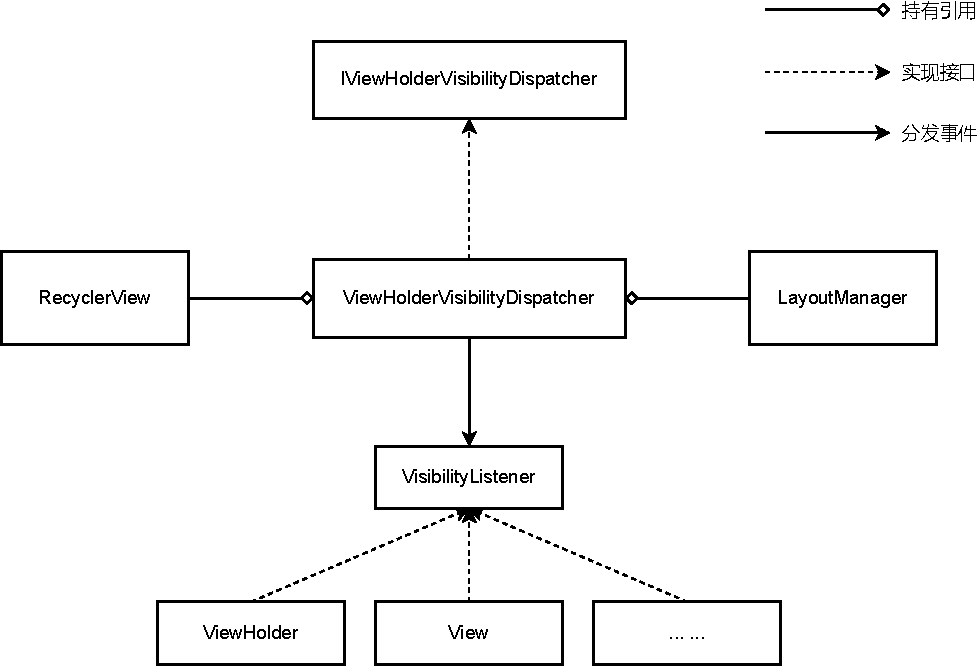
\includegraphics{assets/visibility-dispatch-framework.svg}}

\begin{figure}
    \centering
    \begin{adjustbox}{max width=\textwidth}
        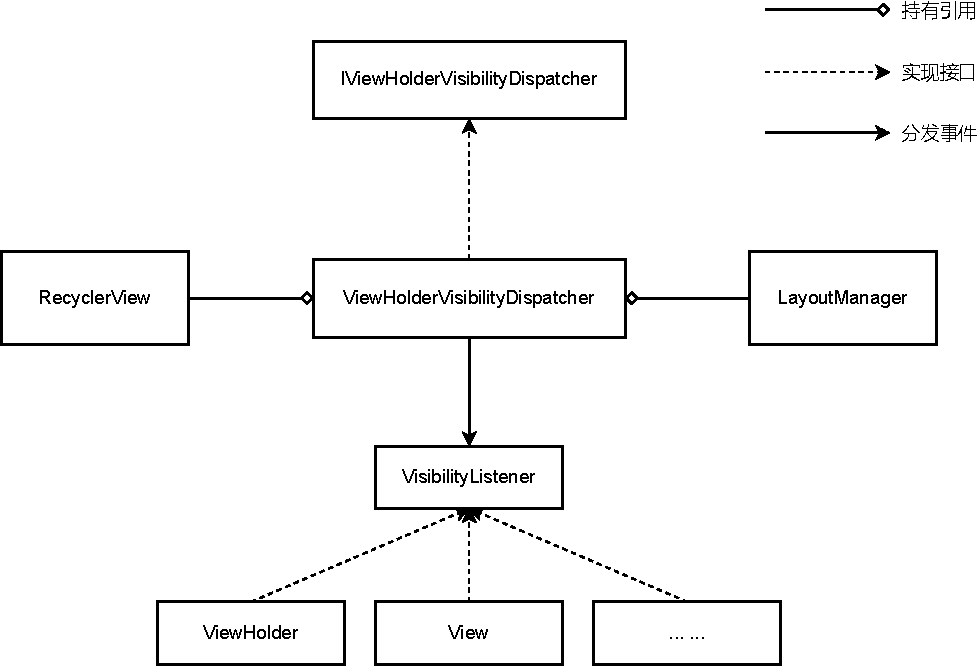
\includegraphics{assets/visibility-dispatch-framework.pdf}
    \end{adjustbox}
    \caption{可见性分发框架设计}
\end{figure}

% 可见性框架的细节

卡片可见性分发的框架设计如图 5.3。ViewHolderVisibilityDispatcher 是主要的卡片可见性事件分发组件,负责核心的可见性计算逻辑以及可见性的记忆和读取操作。由于 RecyclerView 和 LayoutManager 通常在业务中同时初始化,所以将绑定的逻辑也交给 ViewHolderVisibilityDispatcher,让其持有 RecyclerView 和 LayoutManager 的引用,来进行可见性的计算和分发。在相应的时机下,Dispatcher 会将对应的事件分发给 Listener,也就是卡片本身以及监听了可见性事件的业务方组件。在这样的设计模式下,业务方只需要将原来依赖于数据绑定的业务逻辑迁移到新的卡片可见性回调(也就是 VisibilityListener 中的方法)中即可。
\chapter{预渲染框架的缺陷及其修复过程}

在进行预渲染的测试时,发现了一个对性能影响很大,并且很容易触发的缺陷。如果 RecyclerView 的子 View 处理的触摸事件,并且此时有一个依赖于重置布局的动画在不断播放,那么已经被预渲染的卡片就会在滑动屏幕的一瞬间被回收,随后重新绑定。这样的动画在视频 Feed 流中非常常见。如点赞、收藏等互动的动效,一些广告的贴图,一些吸引用户点击的带有动效的按钮等等。由于我们无法规定业务方是否以重置布局的方式编写,所以我们只能默认这种情况很常见。其实不只是动画,任何重置布局的行为在滑动的一瞬间触发,都有可能导致已经被预渲染出的卡片被回收。所以该缺陷产生的原因必须排查清楚,同时需要在改动尽可能小的情况下尝试修复。

卡片被回收的本质,从预渲染的框架设计中就能看出,一定是因为 getExtraLayoutSpace() 返回了默认值0,并且还是要在卡片没有滚动的状态下。只有上述条件全部被满足,RecyclerView 在布局的时候才会因为没有布局到先前预渲染出的卡片,从而将其回收。然而,用户在这个过程中已经传递了 ACTION\_MOVE 事件,意味着滚动行为已经开始。在这个过程中的布局流程,是一定能够布局到预渲染出的卡片的。这代表很可能有其它布局流程在这个过程中被插入到了滚动流程之前,同时 RecyclerView 此时也已经处于滚动状态。顺着这个思路排查,最终注意到了刚才提到的动画。在真实的业务场景中,屏幕上的很多动画都是通过触发布局流程实现的。改变 View 本身的参数,随后调用 requestLayout() 在下一帧中触发布局流程,从而实现动画的效果。这样的动画虽然会影响性能,但是实现简单,同时如果是简单的动效,对于大盘性能的影响不大。所以在大型项目中这样的动画很常见,并且发生的频率也很高。

根据上述发现,怀疑是业务场景中出现的动画影响了 RecyclerView 布局流程,从而导致卡片误回收。然而,在我自己开发的测试项目中进行复现,并没有出现卡片被回收的情况。所以进一步进行调研 RecyclerView 拦截滑动事件、处理滑动事件并设置滚动状态和开始滚动的全链路,找到其中隐藏的问题。

任何 View 处理滑动流程时,都需要处理 ACTION\_DOWN 事件、ACTION\_MOVE 事件和 ACTION\_UP 事件。通常,一个完整的滑动流程是一个 ACTION\_DOWN 加上若干个 ACTION\_MOVE 以及结尾的 ACTION\_UP。因此,对于 RecyclerView 来说,如何处理 ACTION\_DOWN 事件的走向尤为重要,这影响了后续事件的分发,自然也影响了整个的滑动流程。当 ACTION\_DOWN 事件产生时,RecyclerView 并不会拦截该事件,只会将事件传递给子 View。而子 View 可以自主选择是否消费该事件。如果子 View 没有消费 ACTION\_DOWN,那么将会由 RecyclerView 自己来消费。RecyclerView 本身永远会消费任何触摸事件,所以无法再继续向上传递。之后所有的 ACTION\_MOVE 事件以及最后的 ACTION\_UP 事件都会由 RecyclerView 自己来消费。这也是滑动流程中最理想的情况,完全由 RecyclerView 来主动控制。

但是,通常 RecyclerView 的子 View 是需要消费 ACTION\_DOWN 事件的。比如一个可以点击的新闻条目、一个视频条目等等。这些响应了点击事件的子 View 自然需要消费 ACTION\_DOWN 事件来处理点击过程。这也就导致了接下来的 ACTION\_MOVE 事件并不会被发送给 RecyclerView 来消费。那么在这种情况下,RecyclerView 应该如何处理滑动流程呢?答案是通过拦截。虽然 RecyclerView 接下来不会收到子 View 传递来的未经过消费的 ACTION\_MOVE 事件,但是在将其传递给子 View 之前,RecyclerView 本身也可以拦截该事件。因此,RecyclerView 在拦截的流程中,只要发现当前事件是 ACTION\_MOVE 事件,就会设置滑动状态的标记位,并拦截该事件。结果就是子 View 会收到 ACTION\_CANCEL 事件从而无法进行滑动处理(不进行嵌套滑动处理的条件下),而 RecyclerView 本身能够通过该方式消费 ACTION\_MOVE 事件以及最后的 ACTION\_UP 事件。虽然这样确实能够保证 RecyclerView 正常处理滑动流程,但是和直接处理不同,如果是通过拦截的方式处理 ACTION\_MOVE 事件,拦截的过程和真正进行滑动的过程会位于两个不同的消息,也就是两个不同的布局流程中。在这种情况下,如果中间被其他消息插入,就可能会产生一些副作用。

在 RecyclerView 真正进行滑动的过程中,会对每一次滑动事件进行解析。解析出的滑动距离、方向等属性会用于接下来的布局过程。RecyclerView 会对那些因为滑动而改变的子 View 进行重新的测量和布局,并尽可能复用已经被回收的 ViewHolder 来减少重复创建。对于新添加的子 View,也会通过 Adapter 进行数据绑定。

经过以上对源码的分析,我们知道,RecyclerView 在拦截 ACTION\_MOVE 事件时,会设置成滚动状态并拦截该事件。等到下一帧时,会由自己处理触摸事件,从而实现滑动的效果。但是,正是由于设置滚动状态和处理滚动处于不同的消息中,如果有不断触发的重置布局消息,这些消息就可能会被安排在拦截滚动事件和处理滚动事件的消息之间。因为这次布局处于滚动状态,在布局的时候 getExtraLayoutSpace() 就会返回默认值0。由于真实情况是屏幕并没有向下滚动任何距离,所以经过 LayoutManager 计算,已经被渲染出的卡片会被判定为脱离屏幕,从而被回收。

综上所述,如果一个重置布局消息符合以上条件,应该具有如下特点:

\begin{itemize}
    \item RecyclerView 此时处于滚动状态;
    \item 当前处于 RecyclerView 的布局流程,而不是滑动流程;
    \item 屏幕并没有实际向下滚动。
\end{itemize}

根据这三个特点,我们就能够过滤出这样的重置布局消息,并给在这个时机给出额外的布局空间来避免卡片被回收。因此,需要设置 RecyclerView 是否处于布局流程的标记位,并记录本次滑动的滑动方向,通过第一个或者最后一个子 View 的布局参数来判断 RecyclerView 是否已经发生滚动。经过这样的修复,无论是在滚动停止时触发预渲染,还是外界触发的预渲染,都不会再出现已经预渲染的卡片被回收的副作用。
\chapter{预渲染优化验证}

只通过示例无法很好地对优化结果进行验证,同时我们目前还没有一个能够量化的流畅性指标来证明优化的程度。因此需要搭建一个相对真实的视频 Feed 流场景,并在此基础上建立准确、能够量化的流畅性指标来验证预渲染优化对流畅性体验的提升。

\section{搭建视频 Feed 流场景}

视频 Feed 流选用 RecyclerView 搭建,播放器选用谷歌的 Media 库,通过自定义视频展现的 View 来获取视频画面并播放。该案例中,通过解析本地文件夹中的视频,将它们平铺在列表中形成视频 Feed 流。用户上下滑动屏幕,即可与刷短视频一样浏览文件夹中的视频。同时,为了真实模拟短视频应用的体验,开发了沉浸式背景取色、松手起播、视频首帧图像作为视频封面等模块,让整体的体验更加像市面上的短视频应用。

接下来是验证优化结果的过程。为了引入卡顿,在视频卡片的 ViewHolder 绑定过程中人为引入一段耗时逻辑来模拟卡片进行数据绑定时的耗时操作。将视频 Feed 流的 LayoutManager 替换为我们引入了预渲染机制的版本,同时开启不同的模式来体验。我们引入的耗时逻辑越耗时,优化的体验就越明显。具体表现为:在没有预渲染的情况下,每一次滑动都会产生明显的卡顿,并且上滑的动画也出现了不同程度的调帧;在永远预渲染的模式下,只有第一次滑动是流畅的,其它的时候由于额外布局空间永远存在,滑动依然会产生卡顿;在滚动停止触发预渲染的模式下,只有滚动停止时才会进行预渲染,每一次滚动的流畅性都大大增加;在外界触发预渲染的情况下,只有视频开始播放并且滚动已经停止时才会触发预渲染。这意味着只要用户在视频播放之后才滑动屏幕,预渲染的卡片就一直存在,并且预渲染的逻辑也能够避开是视频起播的流程,最大程度地分散耗时任务的布局。

\section{Android 绘制体系的调研}

想要获得准确的流畅性指标,需要对 Android 应用绘制的流程以及其底层的刷新原理非常了解,因此对于这部分内容进行了调研。通过阅读 Android Framework 层和刷新相关的部分源码,总结出了与流畅性相关的绘制流程。

Android 系统底层采用 Skia,OpenGL 等引擎进行绘制,而在上层封装好的组件就是 Canvas 和 View \cite{tahir2013learning}。View绘制系统是 Android 开发者最常用到的 UI 编写 API,同时各种动画、自定义样式等绘制操作也都是交由 View 和 Canvas 来完成。

本课题用到的优化机制,主要是针对 View 的,因此这里着重介绍一下 View 的绘制流程。在 Android 应用中,View 占据了一块屏幕上的矩形区域。在这个区域内,UI 将被显示给用户,同时这块区域也负责处理用户、应用本身输入的事件,从而和用户进行交互。View 的体系非常庞大,绘制系统也非常复杂。这里主要针对 View 的大致分类和普通 View 的绘制流程进行说明。

\subsection{View 的分类}

从总体的功能上看,View 只分为两种:普通的 View 以及 ViewGroup。顾名思义,ViewGroup是用来承载其它 View 和 ViewGroup 的容器;而普通的 View 无法承载其它的 View,只能作为直接和用户交互的组件。在 Android 系统中,View 体系通过树形结构来存储,因此,这棵树上所有的非叶子节点都是 ViewGroup,所有的叶子节点都是普通的 View。

从代码层面来看,ViewGroup 继承自 View,因此 ViewGroup 有着和普通的 View 相似的行为,也需要进行绘制和布局等流程。只不过,ViewGroup 更加关心的是自己内部的子 View 的测量流程,对它们进行统一的管理。\

从内容层级来看,Android 应用程序从最顶层的 DecorView 出发(DecorView 本身被 ViewRootImpl 持有),到持有内容的容器 contentParent,最后到应用开发者主动向 Window 中添加的各种 View,如图 7.1。这些系统级别的 View 一部分是为了管理系统的应用以及悬浮窗等 Window 的通用行为,另一部分是为了给开发者提供额外的扩展能力。因此,我们对于 View 的性能进行优化,主要优化的也是开发者自行添加的这一部分。

% View 层级的图

\begin{figure}
    \centering
    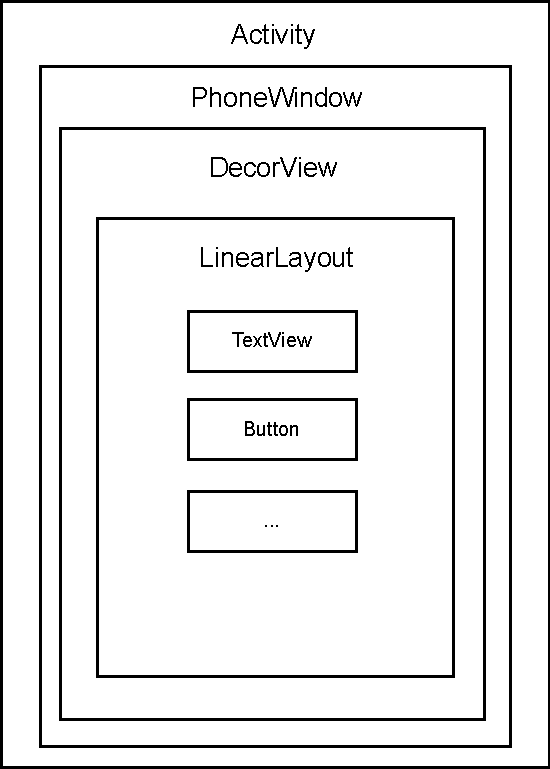
\includegraphics[scale=0.7]{assets/view-hierarchy.pdf}
    \caption{Android 应用程序的 View 层级}
\end{figure}

\subsection{Android 屏幕刷新原理}

在 Android 系统中,屏幕的显示操作需要靠三个部分来完成:CPU,GPU 和显示器。其中,CPU 负责进行绘制信息的计算,其中就包括之后我们介绍的 View 的绘制流程。这些计算好的信息会交给 GPU 进行图形渲染,生成每一个屏幕像素点的颜色信息,并存储到一个缓存当中。当需要让显示器进行显示时,GPU 和显示器的缓存会进行交换,这样显示器得到的就是新的要显示的内容。下面针对屏幕刷新的情况介绍一些概念:

\begin{itemize}
    \item 屏幕刷新率:一秒内屏幕刷新的次数。由于显示器拿到的每一个缓存都包含了屏幕上所有要更新的信息,因此屏幕的显示模式永远是固定的时间将屏幕上的所有像素点进行更新。不过某些情况下,如果前后两次的像素是一致的,那么可以选择不更新,这个操作取决于显示器。因此,即使我们提高了 GPU 将像素信息传送到显示器的速度,屏幕刷新率也是不变的,因为这个指标是对于显示器性能的衡量,而非实际情况;
    \item 逐行扫描:显示器显示像素的原理并不是一次性将缓存中所有的像素点真正更新到屏幕上,而是逐行进行扫描\cite{张春明2002显示器刷新率的测试以及逐行显示器的辨别方法}。因此,这段扫描的时间决定了显示器的素质。通常情况下, Android 手机的显示器扫描一次整个屏幕需要约16.67毫秒。因此,这个时间的结果就是屏幕每秒钟刷新的次数约为60次,也就是屏幕刷新率为60Hz;
    \item 帧率:与屏幕刷新率相对的,帧率表示实际情况下我们传送给显示器的速度。对于运行在 Android 系统的 CPU 来说,这个过程交给了应用的主线程。因此,如果主线程在执行任务的时候过于耗时,没能及时将数据传递给 GPU 和显示器,那么就会让这一帧无法显示在屏幕上,导致屏幕上显示的还是原来的像素,这就是卡顿产生的原因。因此,为了保证真实的帧率能够贴近屏幕刷新率,Android 应用的主线程在处理任务时应该尽可能快,这样才能保证所有的绘制操作顺利进行并最终显示在屏幕上。
\end{itemize}

在某些情况下,屏幕的显示可能会产生抖动。产生这种现象的原因是,当显示器读取缓存,并显示到屏幕上时,GPU 正在向缓存中写入数据。由于并没有做读写保护,所以前后的像素点并不是来自于同一帧。因此后果就是屏幕上的画面产生了撕裂感。解决这种问题的方法是使用双缓存。也就是 GPU 写入的缓存,和显示器读取的缓存并不是同一个。GPU 永远只写入 Back Buffer,显示器只读取 Frame Buffer。而到了需要刷新的时机时,两个缓存的引用会进行交换。由于这个交换的过程非常快,因此可以杜绝绝大部分的画面撕裂问题。

然而,在目前的双缓存机制下,卡顿的问题还是无法得到很好的解决。当 CPU(或者 GPU)在当前帧的持续时间内,无法及时完成图像信息的计算,那么就会发生卡顿。在这种情况下,我们会发现无论是 CPU 还是 GPU,都无法使用 Frame Buffer 或者 Back Buffer。因为前者需要被显示器读取来维持卡顿的帧;后者的数据还没有被显示器读取,等到卡顿帧结束之后,它们还需要被显示到屏幕上。这就导致如果在这个过程中 CPU 和 GPU 有计算任务,计算的结果没有地方保存,也就浪费了 CPU 和 GPU 的绘制时间。针对这个问题,Android 引入了三缓存(Triple Buffering)机制\cite{egilmez2017user}。在三缓存机制下,有两个 Back Buffer 存在,当其中一个因为卡顿而被占用时,CPU 和 GPU 的计算结果就可以存储到另一个缓存中。这样就能有效减少卡顿的传递性带来的连续卡顿。

下一个问题,就是两个缓存进行交换的时机。如果无法保证交换时的读写安全,那么依然会产生显示上的问题。当屏幕的最后一个像素显示完毕后,设备需要一段空闲时间,以便将指针移动回第一个像素来显示下一帧的内容。这段空闲的时间叫做 Vertical Blanking Interval(VBI)。在这段时间内,屏幕上的内容依然会保持原装,并且显示器也不会去读缓存中的内容。因此,这个时间就是进行缓存交换的最佳时刻。在VBI的时间内,系统会发射出用于同步时钟信号的垂直脉冲。这个垂直脉冲也就是 VSync 信号,是我们判断一帧到达的关键信息。

\subsection{Choreographer 和屏幕信号进行同步}

以上的介绍很大程度上是在硬件层面描述 Android 系统中应用的刷新模式。下面我们从软件层面来说明这一过程,来看看在 Android 系统中,画面的刷新流程到底是怎样的。对于应用层的进程来讲,其和屏幕刷新相关的主要媒介是通过一个上层的 Framework 组建 —— Choreographer。

Choreographer 的职责是协调动画、用户输入事件(触摸,外接鼠标等)和绘制流程。它通过底层注册的驱动程序接受系统发出的时间脉冲(也就是上文提到的 VSync 信号),来组织下一帧应该绘制的信息。其中包括让 CPU 去处理下一帧的图像信息,也包括将这些计算好的信息提交给 GPU 来进行渲染。接下来提到的 View 的绘制以及其对于用户输入事件的处理也都是由 Choreographer 在每一帧发起的。

接下来介绍 Choreographer 具体的工作流程。通过之前对于 Android 消息机制的介绍,我们知道,在 Android 应用中,每一个应用的主进程在启动时,都会开启一个 Looper。这个 Looper 的运行函数是一个无限循环,在每一次循环中,会从消息队列中取出一条消息执行,并不断重复这个过程。向 Looper 提供一条消息的方式就是通过另一个组件 —— Handler。Handler 可以发送各种类型的消息,同时具备延时功能。发送的消息会被添加到等待队列中,等待 Looper 将其取出并执行。显然,主线程对应的 Looper 就是主要用来处理各种绘制操作,而绑定了该 Looper 的 Handler 用来向主线程提交各种类型的绘制操作任务。对于 Choreographer,当接收到底层发送的 VSync 信号时,就会向主线程提交一个这样的绘制任务。这就是 Android 应用程序中各种动态界面绘制的源头。

因为这样的绘制机制,我们在开发以及优化应用时,无需关心每一个 VSync 信号实际被发出的时间,只需要关心我们注册的监听器什么时候能接收到 VSync 信号。在这个信号到来时执行绘制的行为,并争取在下一个 VSync 信号到来之前完成它。因此,我们需要区分“帧”和“绘制行为”的区别。通常我们所说的帧指的是每两个 VSync 信号的间隔时间。这段时间内,绘制行为有可能完成,也有可能没有完成;而绘制行为指的是由 Choreographer 发起的从 CPU 到 GPU 最后到显示器的一系列操作。这一串行为在正常情况下只能在一个 VSync 信号到来时开始执行,并在下一个 VSync 信号到来前执行完毕。如果没有及时完成绘制行为,那么下一帧依旧只能显示上一帧的内容,直到绘制完成,缓存可用为止。了解了这些,能够帮助我们在收集流畅性指标时,制定更加精确的收集方案。

Choreographer 在一帧内所做的绘制工作主要有:

\begin{itemize}
    \item 处理用户输入事件;
    \item 处理动画;
    \item 处理 View 的绘制流程。
\end{itemize}

这些绘制工作都作用在应用的 View 树上,通过遍历 View 层级中的各个 View 来对其进行重新绘制,相应触摸之后的新行为等等。在这个过程中,也涉及到很多的性能优化过程,比如增量更新以及脏区计算等等。因此,对于这部分逻辑的改动需要格外小心,确保在优化完毕后,View 的行为对于业务来说和优化之前保持一致。

\section{流畅性指标建设}

能够量化的最直观的流畅性指标就是当前的实时帧率(FPS)。而实时帧率的计算是从 Android 屏幕刷新的过程以及 Choreographer 进行绘制流程得到的。在 API 24 之后,谷歌官方给出了统一的绘制帧情况的收集方法,通过注册 Window 的 onFrameMetricsAvailable() 回调,能够得到绘制的每一帧的信息。通过这些信息,我们能计算当前绘制行为持续的时间等情况,从而计算出帧率和其它的指标。在本案例下,我们计算的指标为长帧占比,即绘制时长超过两个 VSync 间隔的绘制行为在所有绘制行为中的比率。这个指标能够反映当前时间内绘制的流畅程度,长帧占比越高,卡顿的现象就更加严重。

在预渲染关闭和开启的情况下分别统计滑动完所有视频过程中的长帧占比,并控制不同的视频数量,得到如图 7.2 的结果。
    
\begin{figure}[H]
	\centering
		\begin{tikzpicture}
			\begin{axis}[
				xlabel={视频数量(个)},
				ylabel={长帧占比(百分比)},
				xmin=2, xmax=10,
				ymin=8, ymax=18,
				xtick={2, 3, 4, 5, 6, 7, 8, 9, 10},
				ytick={8, 9, 10, 11, 12, 13, 14, 15, 16, 17, 18},
				legend pos=outer north east,
				grid style=dashed,
			]
			
			\addplot[
				color=black,
				mark=square
				]
				coordinates {
				(2,11.11)(3,11.76)(4,14.28)(5,16)(6,17.24)(7,17.14)(8,17.07)(9,17.39)(10,17.3)
				};
			\addlegendentry{预渲染关闭}
		
			\addplot[
				color=black,
				mark=star
				]
				coordinates {
				(2,11.11)(3,11.11)(4,11.11)(5,13.79)(6,14.7)(7,15.38)(8,15.9)(9,15.38)(10,12.67)
				};
			\addlegendentry{一直预渲染}
		
			\addplot[
				color=black,
				mark=diamond
				]
				coordinates {
				(2,8.69)(3,8.51)(4,8.57)(5,8.6)(6,8.62)(7,8.63)(8,8.64)(9,8.64)(10,8.13)
				};
			\addlegendentry{滚动停止预渲染}
		
			\addplot[
				color=black,
				mark=oplus
				]
				coordinates {
				(2,8.33)(3,8.88)(4,8.95)(5,8.98)(6,8.92)(7,8.95)(8,8.97)(9,8.98)(10,8.41)
				};
			\addlegendentry{外界触发预渲染}
			
			\end{axis}
		\end{tikzpicture}
	\caption{流畅性指标折线图}
\end{figure}

在预渲染关闭的情况下,由于每一个视频都需要在滑动的时候进行耗时的数据绑定,因此长帧占比迅速提升到一个平均值并在周围波动;在一直预渲染的情况下,只有滑动到最后一个是视频时,由于不需要预渲染,所以长帧占比大幅度降低,但总体情况依然不理想;在滚动停止预渲染和外界预渲染的情况下,数据绑定不会在滑动的时机进行,所以滑动时的长帧占比大幅度降低。反映到体验上就是用户的滑动会感觉更加流畅。
\chapter{其它形式的优化手段}

\section{View 的异步创建}

Feed 流本身并不局限于视频场景。如微信、今日头条、美团等应用的 Feed 流更多程度上是图文形式、非粘性滑动、具有大量内容的 RecyclerView。在这些场景下,预渲染的思路本身就不适合引入,因为这些场景下屏幕上同时会有非常多的卡片,并且由于非粘性滑动,用户的每一次滑动都不是准确的定位到一个特定的卡片。因此,对于这些场景,更多的优化手段是让首次刷新更加迅速、让卡片创建的耗时尽可能降低等等。本文中主要采用的优化手段为将卡片进行异步创建(Inflate)。

在正常的 RecyclerView 创建卡片时,都是通过 Adapter 的回调实现卡片创建的逻辑。在内部通常会使用布局加载器 LayoutInflater 来通过 XML 文件加载 View。这种方式最耗时的任务就是对于 XML 文件的解析,并根据文件中的 View 层级创建出 View 实例的操作。如果将这部分流程提前进行,在用到的时候直接从缓存池中取用,就能够极大程度地减少 View 创建的耗时。谷歌官方已经提供了将 View 进行异步创建的组件 —— AsyncLayoutInflater。该组件内部拥有一个异步线程以运行业务方提交的 View 加载任务。但是异步创建 View 的难点并不是使用组件进行加载,而是找到加载的时机和用于保存加载出的 View 的缓存。

当 RecyclerView 被初始化时,内部还没有数据。需要等 Adapter 初始化完毕,并主动通知 RecyclerView 数据发生了变化之后,RecyclerView 才会进行相应的布局操作,并在这个过程中将子 View 初始化。在这个过程中,数据到达通常需要等待一段网络 IO 的时间。因此,在这个时间间隔内,我们可以用来进行 View 的异步创建。并且由于 RecyclerView 展示的子 View 的属性通常都是一致的,因此我们可以提前知晓 View 的具体类型,并通知异步的 AsyncLayoutInflater 进行加载;View 的缓存选用 SparseArray。因为 SparseArray 与 HashMap 有相似的结构,所以通过 View 的 id 去访问通常有更高的性能;同时如果需要大量的读写操作,SparseArray 也与队列等结构有相似的效率,比数组在移除、添加操作上有更高的效率。

\section{异步创建优化验证}

为了验证异步创建 View 优化的效果,搭建了一个类似新闻页面的 RecyclerView。此页面在首次刷新时会进行一次假的网络请求,在一段时间之后会返回一些新闻数据,同时用于 Adapter 进行数据绑定并通知 RecyclerView 进行布局。为了模拟 View 创建过程中的耗时行为,人为在子 View 的构造方法中引入耗时逻辑。在这个过程中,开启异步预加载和关闭预加载的情况下,可以明显感觉到有异步创建的时候加载的速度更快。为了进一步量化优化效果,设计了一个“秒开检测框架”:当 RecyclerView 首次刷新时,通过 ViewTreeObserver 的监听器捕获事件,并在回调方法中执行检测逻辑。

秒开框架的检测思路如下:将屏幕分成若干个目标区域。每个区域通过左上角顶点的坐标,以及区域的长和宽来唯一标识。当进行检测时,扫描检测范围内所有的 View,让业务方来决定有效区域的大小。这里的有效区域是指对用户来说有意义的区域大小。以文本类 TextView 来举例子,有效区域就是真实文本所覆盖的区域,不包括四周的留白。当有效区域和屏幕的目标区域的交集超过了一定阈值时,该目标区域被标记为有效;当所有(或大部分)的目标区域都被认为有效时,此时的时刻为页面首次刷新的时长,及秒开时长。该时长标志着应用加载的速度以及给用户带来的体感。时间越短表明对用户来说刷新的感知时间越短,体验越好。

当没有异步创建,以及有异步创建的情况下缓存容量逐渐增加的过程中,缓存个数与秒开时长的关系如下:

这代表如果我们可以针对具体的业务背景选择合适的缓存大小,从而获得最高的首刷流畅性体验。
\end{document}